\section{Embedded system building tools}

\begin{frame}{Approaches}
  Three main approaches to build your embedded Linux system:
  \begin{enumerate}
  \item Cross-compile everything manually from source
  \item Use an {\em embedded Linux build system} that automates the
    cross-compilation process
  \item Use a binary distribution such as Debian, Ubuntu or Fedora
  \end{enumerate}
\end{frame}

\begin{frame}{Approaches pros and cons}
  \begin{center}
  \tiny
  \begin{tabularx}{13cm}{|X|X|X|}
    \hline
    & {\bf Pros} & {\bf Cons} \\
    \hline
    {\bf Building everything manually} &
    Full flexibility \newline
    Learning experience &
    Dependency hell \newline
    Need to understand a lot of details \newline
    Version compatibility \newline
    Lack of reproducibility \\
    \hline
    {\bf Binary distribution} \newline Debian, Ubuntu, Fedora, etc.
    &
    Easy to create and extend \newline
    Extensive set of packages \newline
    Usually excellent security maintenance
    &
    Hard to customize \newline
    Hard to optimize (boot time, size) \newline
    Hard to rebuild the full system from source \newline
    Large system \newline
    Uses native compilation (slow) \newline
    No well-defined mechanism to generate an image \newline
    Lots of mandatory dependencies \newline
    Not available for all architectures \\
    \hline
    {\bf Build systems} \newline Buildroot, Yocto, PTXdist, OpenWrt, etc.
    &
    Nearly full flexibility \newline
    Built from source: customization and optimization are easy \newline
    Fully reproducible \newline
    Uses cross-compilation \newline
    Have embedded specific packages not necessarily in desktop distros \newline
    Make more features optional
    &
    Not as easy as a binary distribution \newline
    Build time \\
    \hline
  \end{tabularx}
  \end{center}
\end{frame}

\subsection{Embedded Linux build systems}

\begin{frame}{Embedded Linux build system: principle}
  \begin{center}
    \includegraphics[width=0.9\textwidth]{slides/sysdev-build-systems/buildsystem-principle.pdf}
  \end{center}
  \begin{itemize}
  \item Building from source $\rightarrow$ lot of flexibility
  \item Cross-compilation $\rightarrow$ leveraging fast build machines
  \item Recipes for building components $\rightarrow$ easy
  \end{itemize}
\end{frame}

\begin{frame}{Build systems vs. Embedded Linux build systems}
  \begin{columns}
    \column{0.6\textwidth}
    \begin{itemize}
    \item Possible confusion between {\em build system} (Makefiles,
      autotools, CMake, Meson) and {\em embedded Linux build systems}
      (Buildroot, Yocto/OpenEmbedded, OpenWrt, etc.)
    \item {\em Build systems} are used by individual software
      components, to control the build process of each source file into
      a library, executable, documentation, etc.
    \item {\em Embedded Linux build systems} are tools that orchestrate
      the build of all software components one after the other. They
      invoke the {\em build system} of each software component.
    \end{itemize}
    \column{0.4\textwidth}
    \begin{center}
      \includegraphics[height=0.8\textheight]{slides/sysdev-build-systems/build-system-vs-embedded-linux-build-system.pdf}
    \end{center}
  \end{columns}
\end{frame}

\begin{frame}{Buildroot: introduction}
  \begin{columns}
    \column{0.2\textwidth}
    
\includegraphics[height=\textwidth,angle=90]{slides/sysdev-build-systems/buildroot-logo.png}
    \column{0.8\textwidth}
    \begin{itemize}
    \item Allows to build a toolchain, a root filesystem image with many
      applications and libraries, a bootloader and a kernel image
      \begin{itemize}
      \item Or any combination of the previous items
      \end{itemize}
    \item Supports building uClibc, glibc and musl toolchains,
      either built by Buildroot, or external
    \item Over 2800 applications or libraries integrated, from basic
      utilities to more elaborate software stacks: Wayland, GStreamer, Qt,
      Gtk, WebKit, Python, PHP, NodeJS, Go, Rust, etc.
    \item Good for small to medium size embedded systems, with a fixed set of
      features
      \begin{itemize}
      \item No support for generating packages (\code{.deb} or
        \code{.ipk})
      \item Needs complete rebuild for most configuration changes.
      \end{itemize}
    \item Active community, releases published every 3 months. One LTS
      release made every year (\code{YYYY.02} so far).
    \end{itemize}
  \end{columns}
\end{frame}

\begin{frame}{Buildroot: configuration and build}
  \begin{columns}
    \column{0.6\textwidth}
    \begin{itemize}
    \item Configuration takes place through a \code{*config} interface similar to the
      kernel\\
      \code{make menuconfig}
    \item Allows to define
      \begin{itemize}
      \item Architecture and specific CPU
      \item Toolchain configuration
      \item Set of applications and libraries to integrate
      \item Filesystem images to generate
      \item Kernel and bootloader configuration
      \end{itemize}
    \item Build:\\
      \code{make}
    \item Useful build results in \code{output/images/}
    \end{itemize}
    \column{0.4\textwidth}
    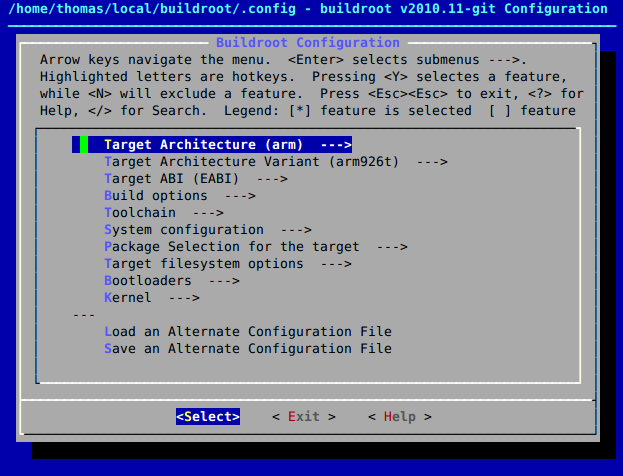
\includegraphics[width=\textwidth]{slides/sysdev-build-systems/buildroot-screenshot.png}
  \end{columns}
\end{frame}

\begin{frame}{Buildroot: adding a new package}
  \begin{itemize}
  \item A package allows to integrate a user application or library to
    Buildroot
  \item Can be used to integrate
    \begin{itemize}
    \item Additional open-source libraries or applications
    \item But also your own proprietary libraries and applications
      $\rightarrow$ fully integrated build process
    \end{itemize}
  \item Each package has its own directory (such as
    \code{package/jose}). This directory contains:
    \begin{itemize}
    \item A \code{Config.in} file (mandatory), describing the
      configuration options for the package. At least one is needed to
      enable the package. This file must be sourced from
      \code{package/Config.in}
    \item A \code{jose.mk} file (mandatory), describing how the
      package is built.
    \item A \code{jose.hash} file (optional, but recommended), containing
      hashes for the files to download, and for the license file.
    \item Patches (optional). Each file of the form
      \code{*.patch} will be applied as a patch.
    \end{itemize}
  \end{itemize}
\end{frame}

\begin{frame}[fragile]{Buildroot: adding a new package, Config.in}
  \begin{block}{package/jose/Config.in}
    {\scriptsize
\begin{verbatim}
config BR2_PACKAGE_JOSE
        bool "jose"
        depends on BR2_TOOLCHAIN_HAS_THREADS
        select BR2_PACKAGE_ZLIB
        select BR2_PACKAGE_JANSSON
        select BR2_PACKAGE_OPENSSL
        help
          C-language implementation of Javascript Object Signing and
          Encryption.

          https://github.com/latchset/jose
\end{verbatim}
      }
    \end{block}

    \begin{block}{package/Config.in}
    {\scriptsize
\begin{verbatim}
[...]
source "package/jose/Config.in"
[...]
\end{verbatim}
    }
    \end{block}
\end{frame}

\begin{frame}[fragile]{Buildroot: adding new package, {\tt .mk} file}
  \begin{block}{package/jose/jose.mk}
    {\scriptsize
\begin{verbatim}
JOSE_VERSION = 11
JOSE_SOURCE = jose-$(JOSE_VERSION).tar.xz
JOSE_SITE = https://github.com/latchset/jose/releases/download/v$(JOSE_VERSION)
JOSE_LICENSE = Apache-2.0
JOSE_LICENSE_FILES = COPYING
JOSE_INSTALL_STAGING = YES
JOSE_DEPENDENCIES = host-pkgconf zlib jansson openssl

$(eval $(meson-package))
\end{verbatim}
      }
    \end{block}
    \begin{itemize}
    \item The package directory and the prefix of all variables must be
      identical to the suffix of the main configuration option
      \code{BR2_PACKAGE_JOSE}
    \item The \code{meson-package} infrastructure knows how to build {\em
        Meson} packages. Many other infrastructures exist, for
      different {\em build systems}
    \end{itemize}
\end{frame}

\begin{frame}{Buildroot resources}
  \begin{columns}
    \column{0.6\textwidth}
    \begin{itemize}
    \item Official site: \url{https://buildroot.org/}
    \item Buildroot manual: \url{https://buildroot.org/downloads/manual/manual.html}
    \item Complete {\em Buildroot system development} training course
      from Bootlin
      \begin{itemize}
      \item \url{https://bootlin.com/training/buildroot/}
      \item Freely available training materials
      \end{itemize}
    \end{itemize}
    \column{0.4\textwidth}
    \begin{center}
      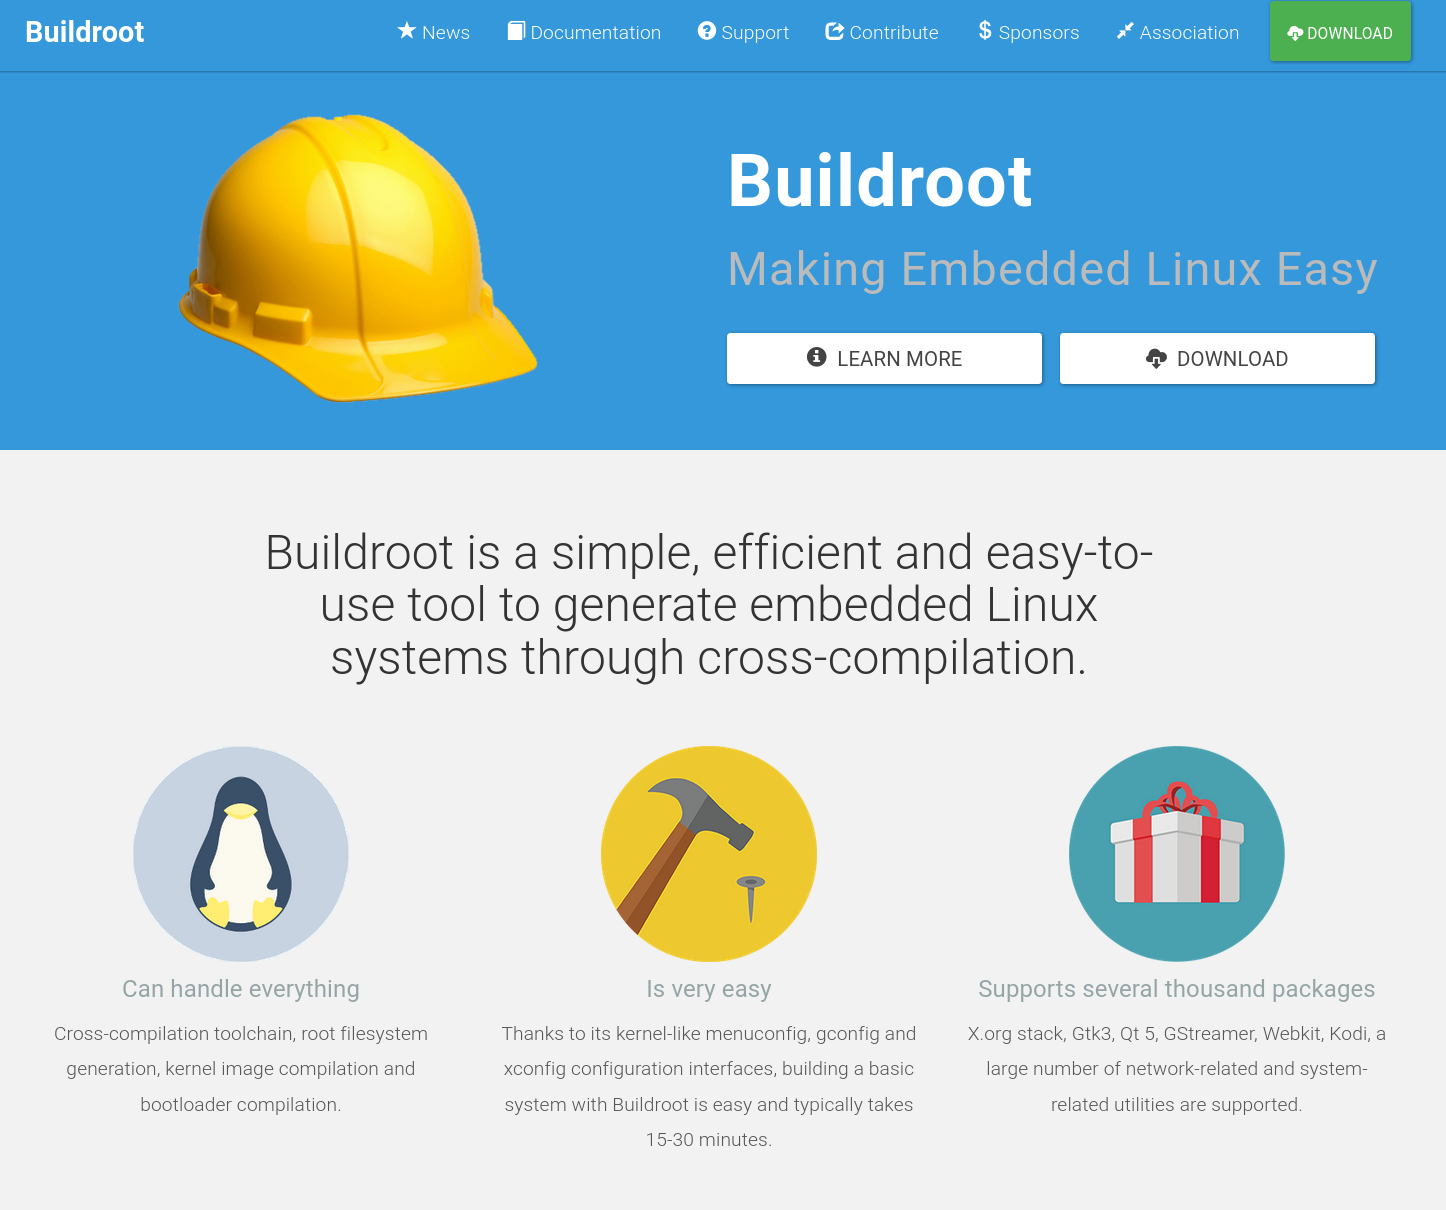
\includegraphics[height=0.4\textheight]{slides/sysdev-build-systems/br-site.png}\\
      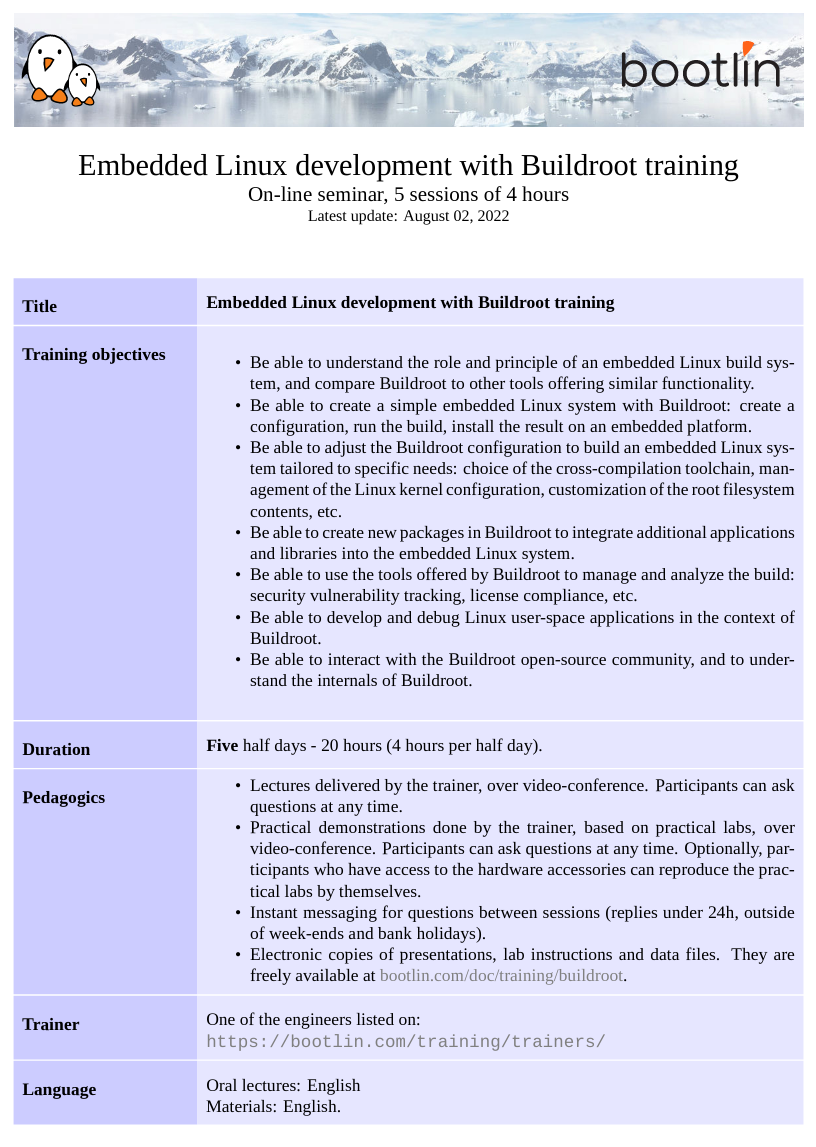
\includegraphics[height=0.4\textheight]{slides/sysdev-build-systems/br-training.png}
    \end{center}
  \end{columns}
\end{frame}

\begin{frame}{Yocto Project / OpenEmbedded}
  \begin{columns}
    \column{0.6\textwidth}
  \begin{itemize}
  \item OpenEmbedded
    \begin{itemize}
    \item Started in 2003
    \item Goal is to build custom Linux distributions for embedded
      devices
    \item Back then, no stable releases, limited/no documentation,
      difficult to use for products
    \end{itemize}
  \item Yocto Project
    \begin{itemize}
    \item Started in 2011
    \item By the Linux Foundation
    \item Goal is to {\em industrialize} OpenEmbedded
    \item Funds the development of OpenEmbedded, makes regular stable
      releases, QA effort, extensive documentation
    \end{itemize}
  \end{itemize}
  \column{0.4\textwidth}
  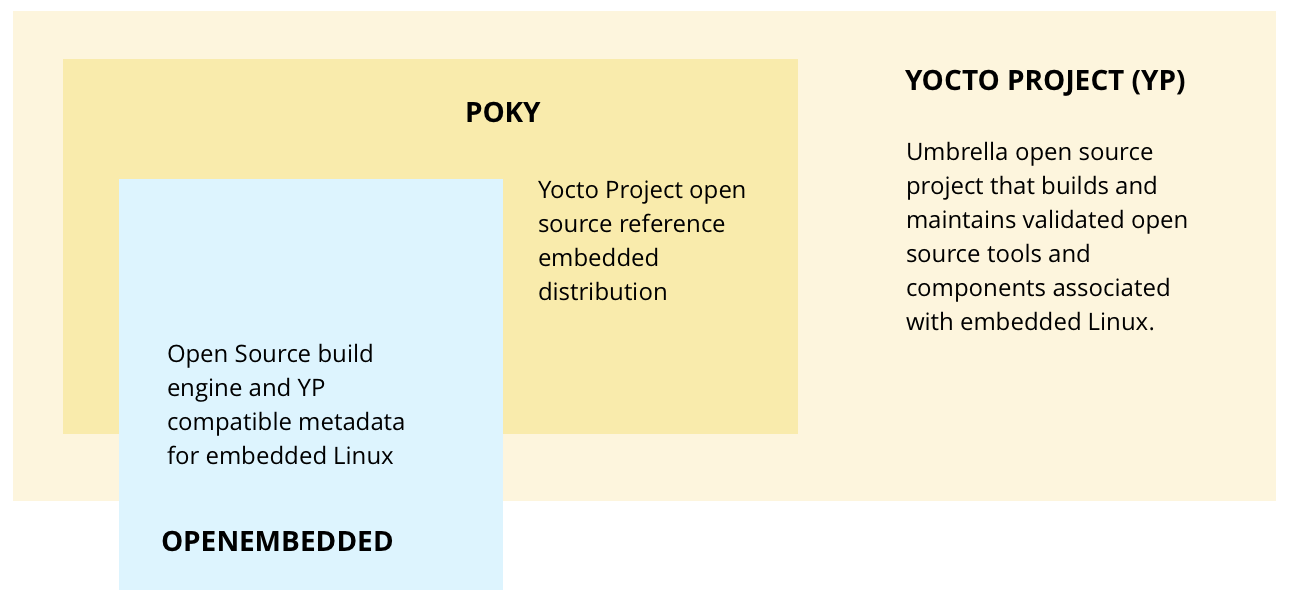
\includegraphics[width=\textwidth]{slides/sysdev-build-systems/yp-diagram-overview.png}
\end{columns}
\end{frame}

\begin{frame}{Yocto Project overview}
  \begin{center}
    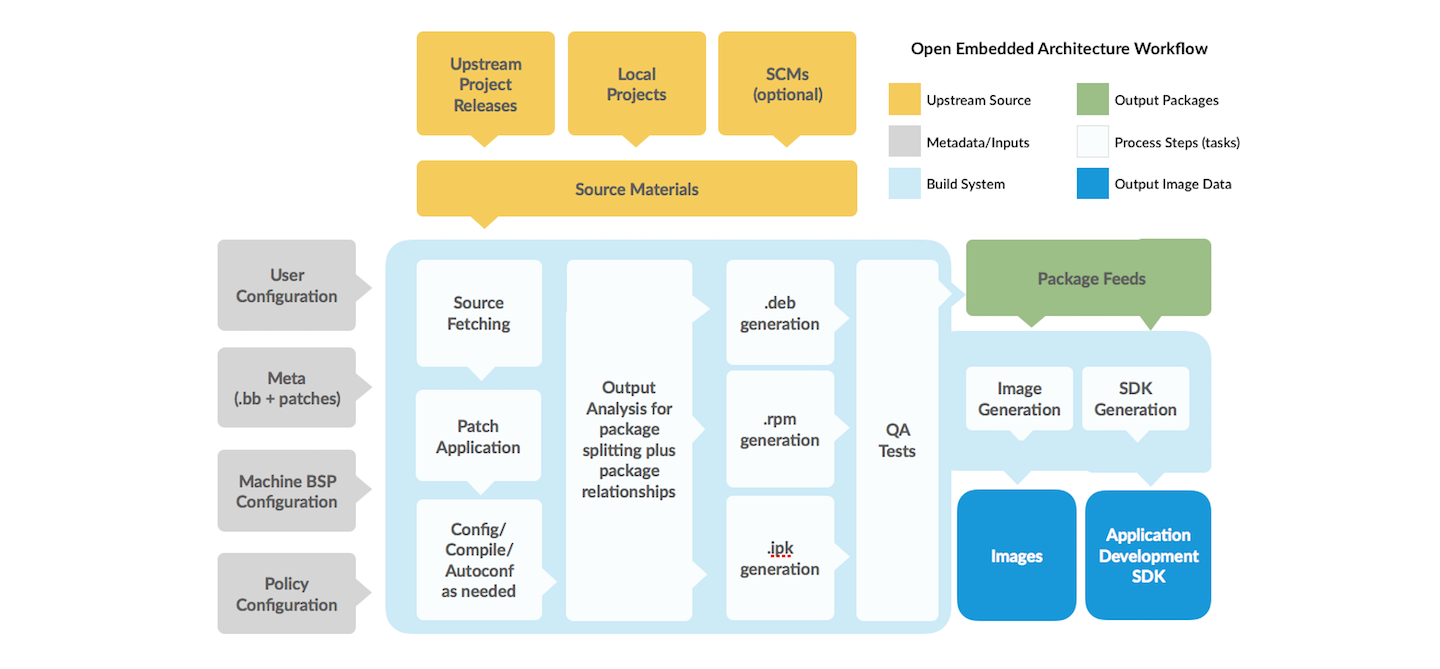
\includegraphics[width=\textwidth]{slides/sysdev-build-systems/yp-how-it-works-new-diagram.png}
  \end{center}
\end{frame}

\begin{frame}{Yocto Project concepts}
  \begin{itemize}
  \item Terminology
    \begin{itemize}
    \item {\bf Layer}: Git repository containing a collection of
      recipes, machines, etc.
    \item {\bf Recipe}: metadata that describes how to build a
      particular software component, the contents of an image to
      generate
    \item {\bf Machine}: a specific hardware platform
    \item {\bf bitbake}: the orchestration tool that processes {\em
        recipes} to generate the final products
    \end{itemize}
  \item Yocto/OpenEmbedded generate a {\em distribution}
    \begin{itemize}
    \item For each recipe, it produces one or several binary packages
      (\code{deb}, \code{rpm}, \code{ipk})
    \item A selection of these binary packages are installed to create
      a {\em root filesystem image} that can be flashed
    \item The other packages can be installed at runtime on the system
      using a package management system: \code{apt}, \code{dnf},
      \code{opkg}
    \end{itemize}
  \end{itemize}
\end{frame}

\begin{frame}{Public layers (1/2)}
  \begin{itemize}
  \item Core layers
    \begin{itemize}
    \item \href{https://git.openembedded.org/bitbake/}{bitbake}, not
      really a layer, but the core build orchestration tool
    \item \href{https://git.openembedded.org/openembedded-core}{openembedded-core},
      the very core recipes, to build the most common software
      packages: Linux, Busybox, toolchain, systemd, mesa3d, X.org,
      bootloaders. Supports only Qemu machines.
    \item \href{https://git.yoctoproject.org/poky/}{poky}, a layer
      from the Yocto Project that combines {\em openembedded-core},
      {\em bitbake}, that defines the {\em Poky} distribution, a
      reference distribution. Supports a few more machines. In
      practice not useful for real projects.
    \item
      \href{http://cgit.openembedded.org/meta-openembedded/}{meta-openembedded},
      community maintained additional recipes from the OpenEmbedded
      project
    \end{itemize}
  \item BSP layers, provided by HW vendors or the community, to
    support additional hardware platforms: recipes for building custom
    Linux kernel, bootloaders, for HW-related software components
    \begin{itemize}
    \item \href{https://git.yoctoproject.org/meta-intel/}{meta-intel},
      \href{https://git.yoctoproject.org/meta-arm/}{meta-arm},
      \href{https://git.yoctoproject.org/meta-ti/}{meta-ti},
      \href{https://git.yoctoproject.org/meta-xilinx/}{meta-xilinx},
      \href{https://git.yoctoproject.org/meta-freescale/}{meta-freescale},
      \href{https://github.com/linux4sam/meta-atmel}{meta-atmel},
      \href{https://github.com/STMicroelectronics/meta-st-stm32mp}{meta-st-stm32mp},
      etc.
    \end{itemize}
  \end{itemize}
\end{frame}

\begin{frame}{Public layers (2/2)}
  \begin{itemize}
  \item Additional software layers: recipes for building additional
    software components, not in {\em openembedded-core}
    \begin{itemize}
    \item
      \href{https://code.qt.io/cgit/yocto/meta-qt6.git/}{meta-qt6},
      \href{https://git.yoctoproject.org/meta-virtualization}{meta-virtualization},
      \href{https://github.com/rauc/meta-rauc}{meta-rauc},
      \href{https://github.com/sbabic/meta-swupdate}{meta-swupdate},
      etc.
    \end{itemize}
  \item Layer index: \url{https://layers.openembedded.org/}
  \item Each layer normally has a branch matching the Yocto release
    you're using
  \item Not all layers have the same level of quality/maintenance:
    third-party layers are not necessarily reviewed by OpenEmbedded
    experts.
  \end{itemize}
\end{frame}

\begin{frame}{Combine layers}
  \begin{itemize}
  \item For your project, you will typically combine a number of
    public layers
    \begin{itemize}
    \item At least the {\em openembedded-core} layer
    \item Possibly one or several {\em BSP layers}
    \item Possibly one or several additional {\em software layers}
    \end{itemize}
  \item And you will create your {\em own layer}, containing recipes
    for:
    \begin{itemize}
    \item Machine definitions for your custom hardware platforms
    \item Image/distro definitions for your custom system(s)
    \item Recipes for your custom software
    \end{itemize}
  \item A tool is often used to automate the retrieval of the
    necessary layers, at the right version
    \begin{itemize}
    \item \href{https://gerrit.googlesource.com/git-repo/}{Google
        repo} tool, the Yocto-specific
      \href{https://kas.readthedocs.io}{Kas} utility
    \end{itemize}
  \end{itemize}
\end{frame}

\begin{frame}[fragile]{Yocto quick start: STM32MP1 example}
  \begin{block}{Download {\em bitbake} and layers}
    {\footnotesize
\begin{verbatim}
  $ git clone git://git.openembedded.org/openembedded-core -b kirkstone
  $ git clone git://git.openembedded.org/meta-openembedded -b kirkstone
  $ git clone git://git.openembedded.org/bitbake -b 2.0
  $ git clone https://github.com/STMicroelectronics/meta-st-stm32mp.git -b kirkstone
\end{verbatim}
    }
  \end{block}

  Note: we're not using a tool such as {\em repo} or {\em Kas} here,
  we are fetching each layer manually.

  \begin{block}{Enter the build environment}
    {\footnotesize
\begin{verbatim}
$ source openembedded-core/oe-init-build-env
\end{verbatim}
    }
  \end{block}

  This automatically enters a directory called \code{build/}, with a
  few files/directories already prepared.
\end{frame}

\begin{frame}[fragile]{Yocto quick start: STM32MP1 example}
  \begin{block}{Configure layers: {\em conf/bblayers.conf}}
    {\footnotesize
\begin{verbatim}
BBLAYERS ?= " \
  /path/to/openembedded-core/meta \
  /path/to/meta-st-stm32mp \
  /path/to/meta-openembedded/meta-oe \
  /path/to/meta-openembedded/meta-python \
  "
\end{verbatim}
    }
  \end{block}

  \begin{block}{Start the build}
    {\footnotesize
\begin{verbatim}
$ MACHINE=stm32mp1 bitbake core-image-minimal
\end{verbatim}
    }
  \end{block}

  \begin{itemize}
  \item \code{MACHINE=stm32mp1} will build images usable on all
    STM32MP1 platforms
  \item \code{core-image-minimal} builds a minimal image
  \end{itemize}

  \begin{block}{Build results}
    {\footnotesize
\begin{verbatim}
$ ls tmp/deploy/images/stm32mp1/
\end{verbatim}
    }
  \end{block}
\end{frame}

\begin{frame}[fragile]{Yocto recipe example}
  \begin{block}{{\tt
\href{https://git.openembedded.org/openembedded-core/tree/meta/recipes-extended/libmnl/libmnl_1.0.5.bb}
     {openembedded-core/tree/meta/recipes-extended/libmnl/libmnl\_1.0.5.bb}}}
    {\tiny
\begin{verbatim}
SUMMARY = "Minimalistic user-space Netlink utility library"
DESCRIPTION = "Minimalistic user-space library oriented to Netlink developers, providing \
    functions for common tasks in parsing, validating, and constructing both the Netlink header and TLVs."
HOMEPAGE = "https://www.netfilter.org/projects/libmnl/index.html"
SECTION = "libs"
LICENSE = "LGPL-2.1-or-later"
LIC_FILES_CHKSUM = "file://COPYING;md5=4fbd65380cdd255951079008b364516c"

SRC_URI = "https://netfilter.org/projects/libmnl/files/libmnl-${PV}.tar.bz2"
SRC_URI[sha256sum] = "274b9b919ef3152bfb3da3a13c950dd60d6e2bcd54230ffeca298d03b40d0525"

inherit autotools pkgconfig

BBCLASSEXTEND = "native"
\end{verbatim}
    }
  \end{block}
  \begin{itemize}
  \item Recipe to build
    \href{https://www.netfilter.org/projects/libmnl/}{libmnl}
  \item Build system based on {\em autotools} $\rightarrow$
    \code{inherit autotools}
  \item Available both for the target and the host $\rightarrow$
    \code{BBCLASSEXTEND = "native"}
  \end{itemize}
\end{frame}

\begin{frame}{Yocto resources}
  \begin{columns}
    \small
    \column{0.6\textwidth}
    \begin{itemize}
    \item Official website: \url{https://www.yoctoproject.org/}
    \item Release information:\\
          \url{https://wiki.yoctoproject.org/wiki/Releases}
    \item Official documentation: \url{https://docs.yoctoproject.org/}
      \begin{itemize}
      \item Maintained by Bootlin engineers!
      \end{itemize}
    \item Complete {\em Yocto Project and OpenEmbedded system
        development} training course from Bootlin
      \begin{itemize}
      \item \url{https://bootlin.com/training/yocto/}
      \item Freely available training materials
      \end{itemize}
    \end{itemize}
    \column{0.4\textwidth}
    \begin{center}
      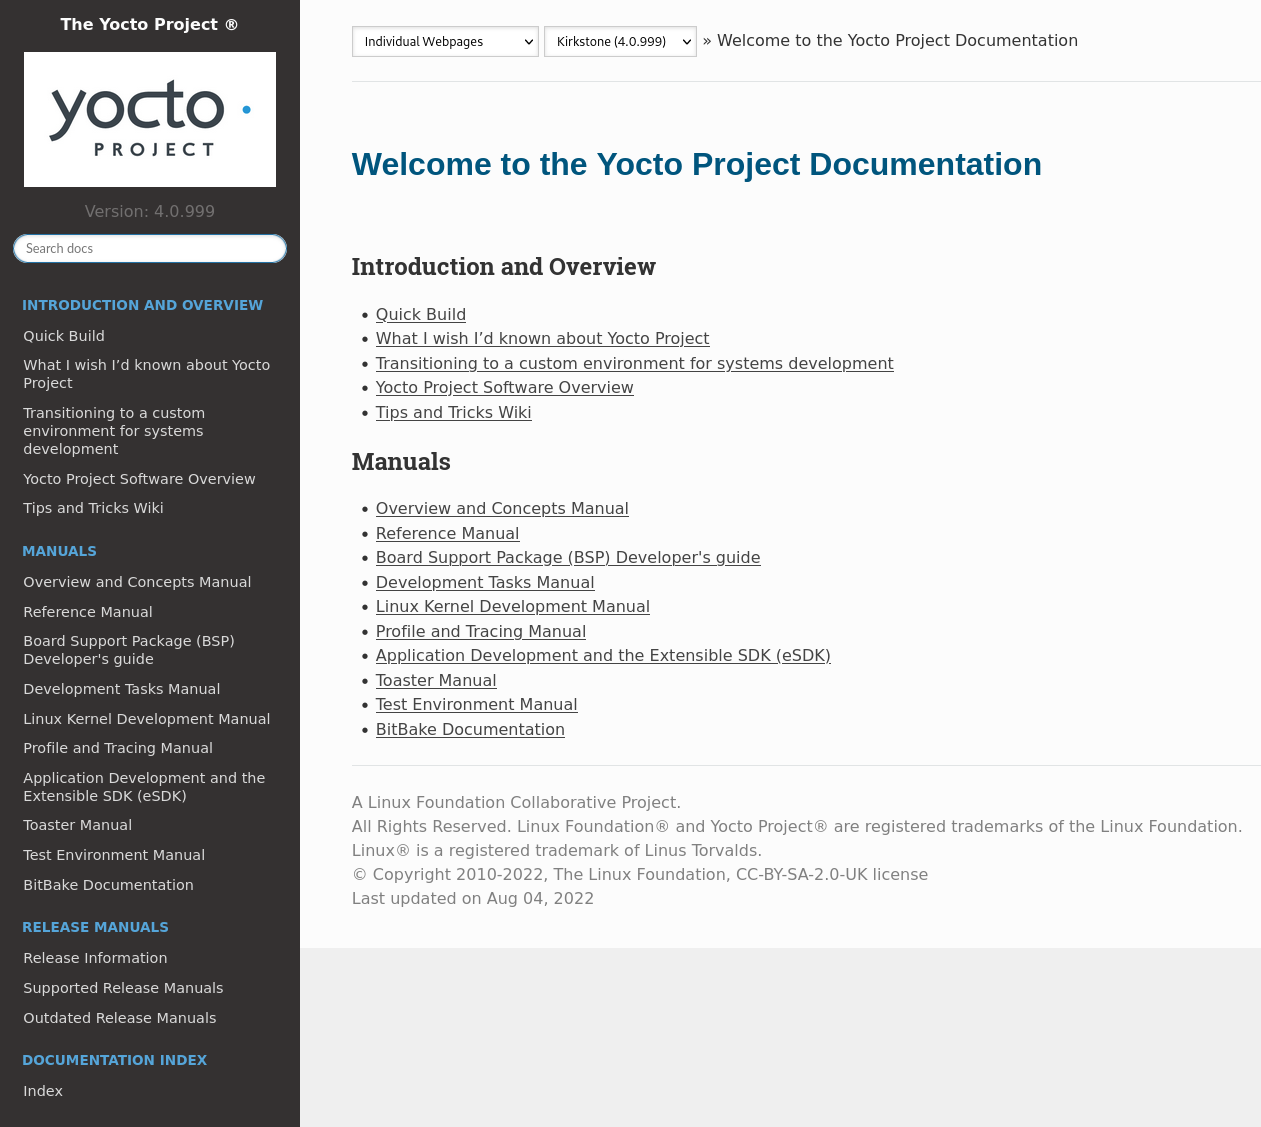
\includegraphics[height=0.4\textheight]{slides/sysdev-build-systems/yp-docs.png}\\
      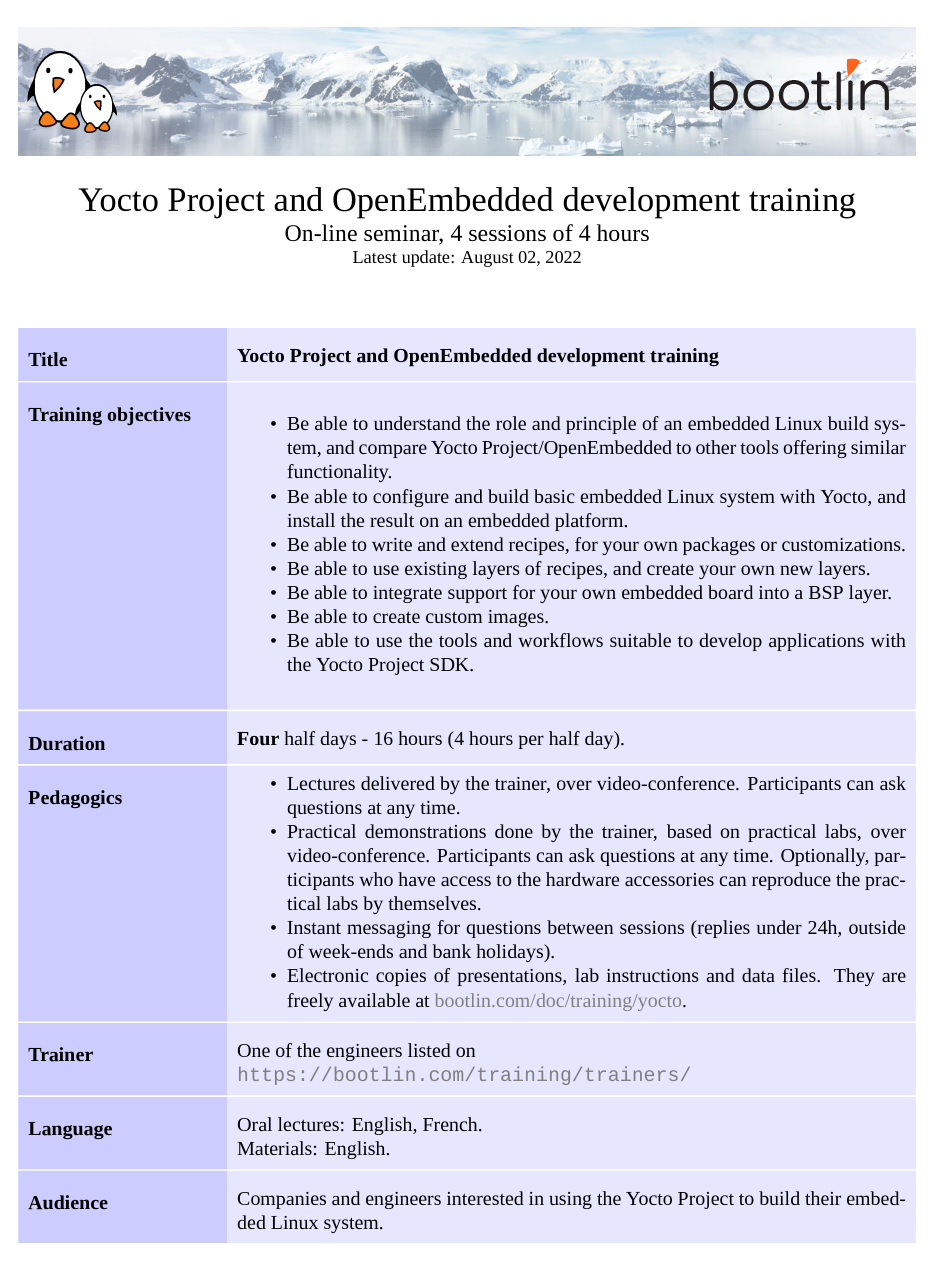
\includegraphics[height=0.4\textheight]{slides/sysdev-build-systems/yp-training.png}
    \end{center}
  \end{columns}
\end{frame}

\begin{frame}{Buildroot vs. Yocto: a few key differences}
  \begin{itemize}
  \item What it builds
    \only<1> {
      \begin{itemize}
      \item {\bf Yocto}: builds a distribution, with binary packages and a
        package management system
      \item {\bf Buildroot}: builds a fixed functionality root
        filesystem, no binary packages
      \item Note: binary packages are not necessarily a good thing for
        embedded!
      \end{itemize}
    }
    \pause
  \item Configuration
    \only<2> {
      \begin{itemize}
      \item {\bf Yocto}: flexible, powerful but complex configuration
        description
      \item {\bf Buildroot}: very simple configuration system, but
        sometimes limited
      \end{itemize}
    }
    \pause
  \item Build strategy
    \only<3> {
      \begin{itemize}
      \item {\bf Yocto}: complex and heavy logic, but with efficient
        caching of artifacts and ``rebuild only what's needed'' features
      \item {\bf Buildroot}: simple but somewhat dumb logic, no caching
        of built artifacts, full rebuilds needed for some config changes
      \end{itemize}
    }
    \pause
  \item Ecosystem
    \only<4> {
      \begin{itemize}
      \item {\bf Yocto}: (relatively) small common base in OpenEmbedded,
        lots of features supported in third party layers $\rightarrow$
        lots of things, but varying quality
      \item {\bf Buildroot}: everything in one tree $\rightarrow$
        perhaps less things, but more consistent quality
      \end{itemize}
    }
    \pause
  \item Complexity/learning curve
    \only<5> {
      \begin{itemize}
      \item {\bf Yocto}: admittedly steep learning curve, {\em bitbake}
        remains a magic black box for most people
      \item {\bf Buildroot}: much smoother and shorter learning curve,
        the tool is simple to approach, and reasonably simple to
        understand
      \end{itemize}
    }
    \pause
  \item And also a matter of personal taste/preference, as often when
    choosing tools
  \end{itemize}
\end{frame}

\begin{frame}{OpenWrt}
  \begin{itemize}
  \item Another Embedded Linux build system
  \item Derived from Buildroot a {\em very} long time ago
    \begin{itemize}
    \item Now completely different, except for the use of {\em Kconfig} and {\em make}
    \end{itemize}
  \item Targeted at building firmware for WiFi routers and other
    networking equipments
  \item Unlike Buildroot or Yocto that leave a lot of flexibility to
    the user in defining the system architecture, OpenWrt makes a lot
    of set in stone decisions:
    \begin{itemize}
    \item {\em musl} is the C library
    \item an OpenWrt specific init system
    \item an OpenWrt specific inter-process communication bus
    \item a Web UI specific to OpenWrt
    \end{itemize}
  \item The aim of OpenWrt is to build a final product out of the box,
    with support for popular networking products and development
    boards
  \item \code{https://openwrt.org/}
  \end{itemize}
\end{frame}

\subsection{Working with distributions}

\begin{frame}{Binary distributions}
  \begin{itemize}
  \item Many popular Linux desktop/server distributions have support
    for embedded architectures
    \begin{itemize}
    \item \href{https://www.debian.org}{Debian}: ARMv5, ARMv7, ARM64,
      i386, x86-64, MIPS, PowerPC, RISC-V in progress
    \item \href{https://www.ubuntu.com}{Ubuntu}: ARMv7, ARM64,
      x86-64, RISC-V (initial support), PowerPC64 little-endian
    \item \href{https://getfedora.org}{Fedora}: ARMv7, ARM64, x86-64,
      MIPS little-endian, PowerPC64 little-endian, RISC-V
    \end{itemize}
  \item Some more specialized Linux distributions as well
    \begin{itemize}
    \item \href{https://www.raspberrypi.com/software/}{Raspberry Pi
        OS}, a Debian derivative targeted at RaspberryPi platforms
    \item \href{https://www.alpinelinux.org/}{Alpine Linux}, a
      lightweight distribution, based on {\em musl} and {\em Busybox},
      ARMv7, ARM64, i386, x86-64, PowerPC64 little-endian
    \end{itemize}
  \end{itemize}
\end{frame}

\begin{frame}{Binary distributions pitfalls}
  \begin{itemize}
  \item Be careful when using a binary distribution on how you create
    your system image, and how reproducible this process is
  \item We have seen projects use the following (bad) procedure:
    \begin{itemize}
    \item Install a binary distribution manually on their target hardware
    \item Install all necessary packages by hand
    \item Compile the final applications on the target
    \item Tweak configuration files directly on the target
    \item Then duplicate the resulting SD card for all other boards
    \end{itemize}
  \item This process is really bad as:
    \begin{itemize}
    \item it is not reproducible
    \item it requires installing many more things on the target than
      needed (development tools), increasing the footprint, the attack
      surface and the maintenance effort
    \end{itemize}
  \item If you end up using a binary distribution in production, make
    sure you have an automated and reproducible process to generate
    the complete image, ready to flash on your target.
  \end{itemize}
\end{frame}

\begin{frame}{Debian/Ubuntu image building tools}
  \begin{columns}
    \column{0.6\textwidth}
    ELBE
    \begin{itemize}
    \item {\bf E.}mbedded {\bf L.}inux {\bf B.}uild {\bf E.}nvironment
    \item Implemented in Python
    \item Uses an XML file as input to describe the system to generate
    \item Can use pre-built packages from Debian/Ubuntu repositories,
      but can also cross-compile and install additional packages
    \item \url{https://elbe-rfs.org/}
    \item \href{https://www.youtube.com/watch?v=BwHzyCGB7As}{Building
        Embedded Debian and Ubuntu Systems with ELBE} talk
    \item
      \href{https://bootlin.com/blog/elbe-automated-building-of-ubuntu-images-for-a-raspberry-pi-3b/}{ELBE:
        automated building of Ubuntu images for a Raspberry Pi 3B}
    \end{itemize}
    \column{0.4\textwidth}
    DebOS
    \begin{itemize}
    \item Debian OS images builder
    \item Implemented in Go
    \item Uses a YAML file as input to describe the system to generate
    \item \href{https://www.youtube.com/watch?v=_NZrSR3prwk}{Creating
        Debian-Based Embedded Systems in the Cloud Using Debos} talk
    \item \url{https://github.com/go-debos/debos}
    \end{itemize}
  \end{columns}
\end{frame}

\begin{frame}{Android}
  \begin{itemize}
  \item The obviously highly popular mobile operating system
  \item Uses the Linux kernel
  \item Most of the user-space is completely different from a normal
    embedded Linux system
    \begin{itemize}
    \item Most components rewritten by Google
    \item {\em bionic} C library
    \item Custom {\em init} system and device management
    \item Custom IPC mechanism, custom display stack, custom
      multimedia stack
    \item Custom build system
    \end{itemize}
  \item Android pitfalls for industrial embedded systems
    \begin{itemize}
    \item Large footprint, and resource hungry
    \item Complexity and build time
    \item Maintenance issues: difficult to upgrade to newer releases
      due to increasing hardware requirements
    \end{itemize}
  \item
    \href{https://www.opersys.com/training/embedded-android-training/}{Embedded
      Android Training} course from
    \href{https://www.opersys.com}{Opersys}, with freely available
    training materials
  \end{itemize}
\end{frame}

\begin{frame}{Automotive Grade Linux, Tizen}
  \begin{itemize}
  \item Industry groups collaborate around the creation of embedded
    Linux distributions targeting specific markets
    \begin{itemize}
    \item These are regular embedded Linux systems, usually based on
      Yocto, with a selection of relevant open-source software components
    \item Fund the development of missing features in existing
      components, or development of new software components
    \end{itemize}
  \item Automotive Grade Linux
    \begin{itemize}
    \item Linux Foundation project
    \item {\em Collaborative open source project that is bringing
        together automakers, suppliers and technology companies to
        accelerate the development and adoption of a fully open
        software stack for the connected car}
    \item \url{https://www.automotivelinux.org/}
    \end{itemize}
  \item Tizen
    \begin{itemize}
    \item {\em Tizen is an open and flexible operating system built
        from the ground up to address the needs of all stakeholders of
        the mobile and connected device ecosystem}
    \item \url{https://www.tizen.org/}
    \end{itemize}
  \end{itemize}
\end{frame}

\setuplabframe
{System build with Buildroot}
{
  Time to start the practical lab!
  \begin{itemize}
  \item Using Buildroot to rebuild the same basic system plus a sound
    playing server ({\em MPD}) and a client to control it ({\em mpc}).
  \item Overlaying the root filesystem built by Buildroot
  \item Driving music playback, directly from the target, and then
    remotely through an MPD client on the host machine.
  \item Analyzing dependencies between packages.
  \item Building {\em evtest} and using it to test the Nunchuk
	device driver.
  \end{itemize}
}
